\documentclass[11pt]{article}
\usepackage{amsmath}
\usepackage{amssymb}
\usepackage{graphicx}
\usepackage{fancyhdr}
\usepackage{enumerate}
\usepackage{enumitem}
\usepackage{float}
\usepackage[colorlinks=true,urlcolor=blue]{hyperref}

% No page numbers
%\pagenumbering{gobble}

% MARGINS (DO NOT EDIT) ---------------------------------------------
\oddsidemargin  0in \evensidemargin 0in \topmargin -0.5in
\headheight 0.25in \headsep 0.25in
\textwidth   6.5in \textheight 9in
\parskip 1.5ex  \parindent 0ex \footskip 20pt
% ---------------------------------------------------------------------------------

% HEADER (DO NOT EDIT) -----------------------------------------------
\newcommand{\problemnumber}{0}
\newcommand{\myname}{name}
\newfont{\myfont}{cmssbx10 scaled 1200}
\pagestyle{fancy}
\fancyhead{}
\fancyhead[L]{\myfont Question \problemnumber, Assignment 2, CS224n}
%\fancyhead[R]{\bssnine \myname}
\newcommand{\newquestion}[1]{
\clearpage % page break and flush floats
\renewcommand{\problemnumber}{#1} % set problem number for header
\phantom{}  % Put something on the page so it shows
}
% ---------------------------------------------------------------------------------

% BEGIN HOMEWORK HERE
\begin{document}

% Question 1
\newquestion{1}
\begin{enumerate}[label=(\alph*)]
    \item It's intuitive that only when $w$ equals to $o$, $y_w$ wont be 0.
    \item First, we have $\hat{y} =  softmax(U^Tv_c)$. Then
    \begin{equation*}
        \begin{aligned}
            \frac{\partial J}{\partial v_c} 
            &= \frac{\partial J}{\partial U^Tv_c} \frac{\partial U^Tv_c}{\partial v_c} \\
            &= U^T(\hat{y} - y)
        \end{aligned}
    \end{equation*}
    \item The first steps are the same as the last problem. We have $\hat{y} = softmax(U^Tv_c)$. Then
    \begin{equation*}
        \begin{aligned}
            \frac{\partial J}{\partial u_w} 
            &= \frac{\partial J}{\partial U^Tv_c} \frac{\partial U^Tv_c}{\partial u_w} \\
            &= v_c (\hat{y} - y)^T
        \end{aligned}
    \end{equation*}
    \item The process is as below,
    \begin{equation*}
        \begin{aligned}
            \frac{\partial \sigma(x)}{\partial x} 
            &= \frac{e^x(e^x+1) - e^x e^x}{\partial (e^x+1)^2} \\
            &= \sigma(x)(1-\sigma(x))
        \end{aligned}
    \end{equation*}
    \item The partial derivative for $v_c$ is $$(\sigma (u_o^Tv_c)-1)u_o + \sum_{k=1}^K(\sigma(-u_k^Tv_c)-1)u_k$$.\\
    The partial derivative for $u_o$ is $$(\sigma (u_o^Tv_c)-1)v_c$$ and for $u_k$ is $$(\sigma(-u_k^Tv_c)-1)v_c$$. \\
    This derivative is easier to compute because we don't need to compute the partial derivative for all words in vocabulary. \\
    \item 
    \begin{enumerate}[label=(\roman*)]
        \item $\sum_{j \in window} \frac{\partial J(v_c,w_j,U)}{\partial U}$
        \item $\sum_{j \in window} \frac{\partial J(v_c,w_j,U)}{\partial v_c}$
        \item 0
    \end{enumerate}
\end{enumerate}


\newquestion{2}
After training, final loss is 9.367644. \\
The results of word vectors are as shown in the belowing picture.
\begin{figure}[H]
    \centering
    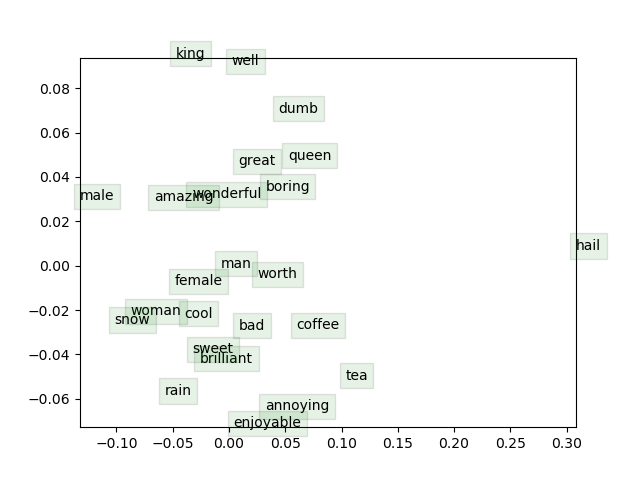
\includegraphics[width=0.80\textwidth]{pic/word_vectors.png}
    \caption{word vectors}
\end{figure}
We can see that
\begin{enumerate}
    \item Some words like amazing, wonderful and boring are clustered well
    \item Some words like hail, snow and rain are not.
    \item It's interesting to see that the relative distance between male to king and female to queen is equal.
\end{enumerate}

\end{document}
